\documentclass[prb,preprint]{revtex4-1} 
% The line above defines the type of LaTeX document.
% Note that AJP uses the same style as Phys. Rev. B (prb).

\usepackage{amsmath}  % needed for \tfrac, \bmatrix, etc.
\usepackage{amsfonts} % needed for bold Greek, Fraktur, and blackboard bold
\usepackage{graphicx} % needed for figures

\begin{document}

% Be sure to use the \title, \author, \affiliation, and \abstract macros
% to format your title page.  Don't use lower-level macros to  manually
% adjust the fonts and centering.

\title{Measuring the Verdet Constant in XXXXX}


\author{Liza Mulder}
\email{emulder@smith.edu}
\affiliation{Department of Physics, Smith College, Northampton, MA 01063}


\author{Danika Luntz-Martin}
\email{dluntzma@smith.edu}
\affiliation{Department of Physics, Smith College, Northampton, MA 01063}


\date{\today}



\begin{abstract}

\end{abstract}

\maketitle % title page is now complete


\section{Introduction} % Section titles are automatically converted to all-caps.
% Section numbering is automatic.

\section{Methods}

Our experimental setup was based off the TeachSpin teaching manual. We used a TeachSpin XXXX consisting of a diode laser, a solenoid, a polarizing lens and photodetector. 

\begin{figure}[h!]
\centering
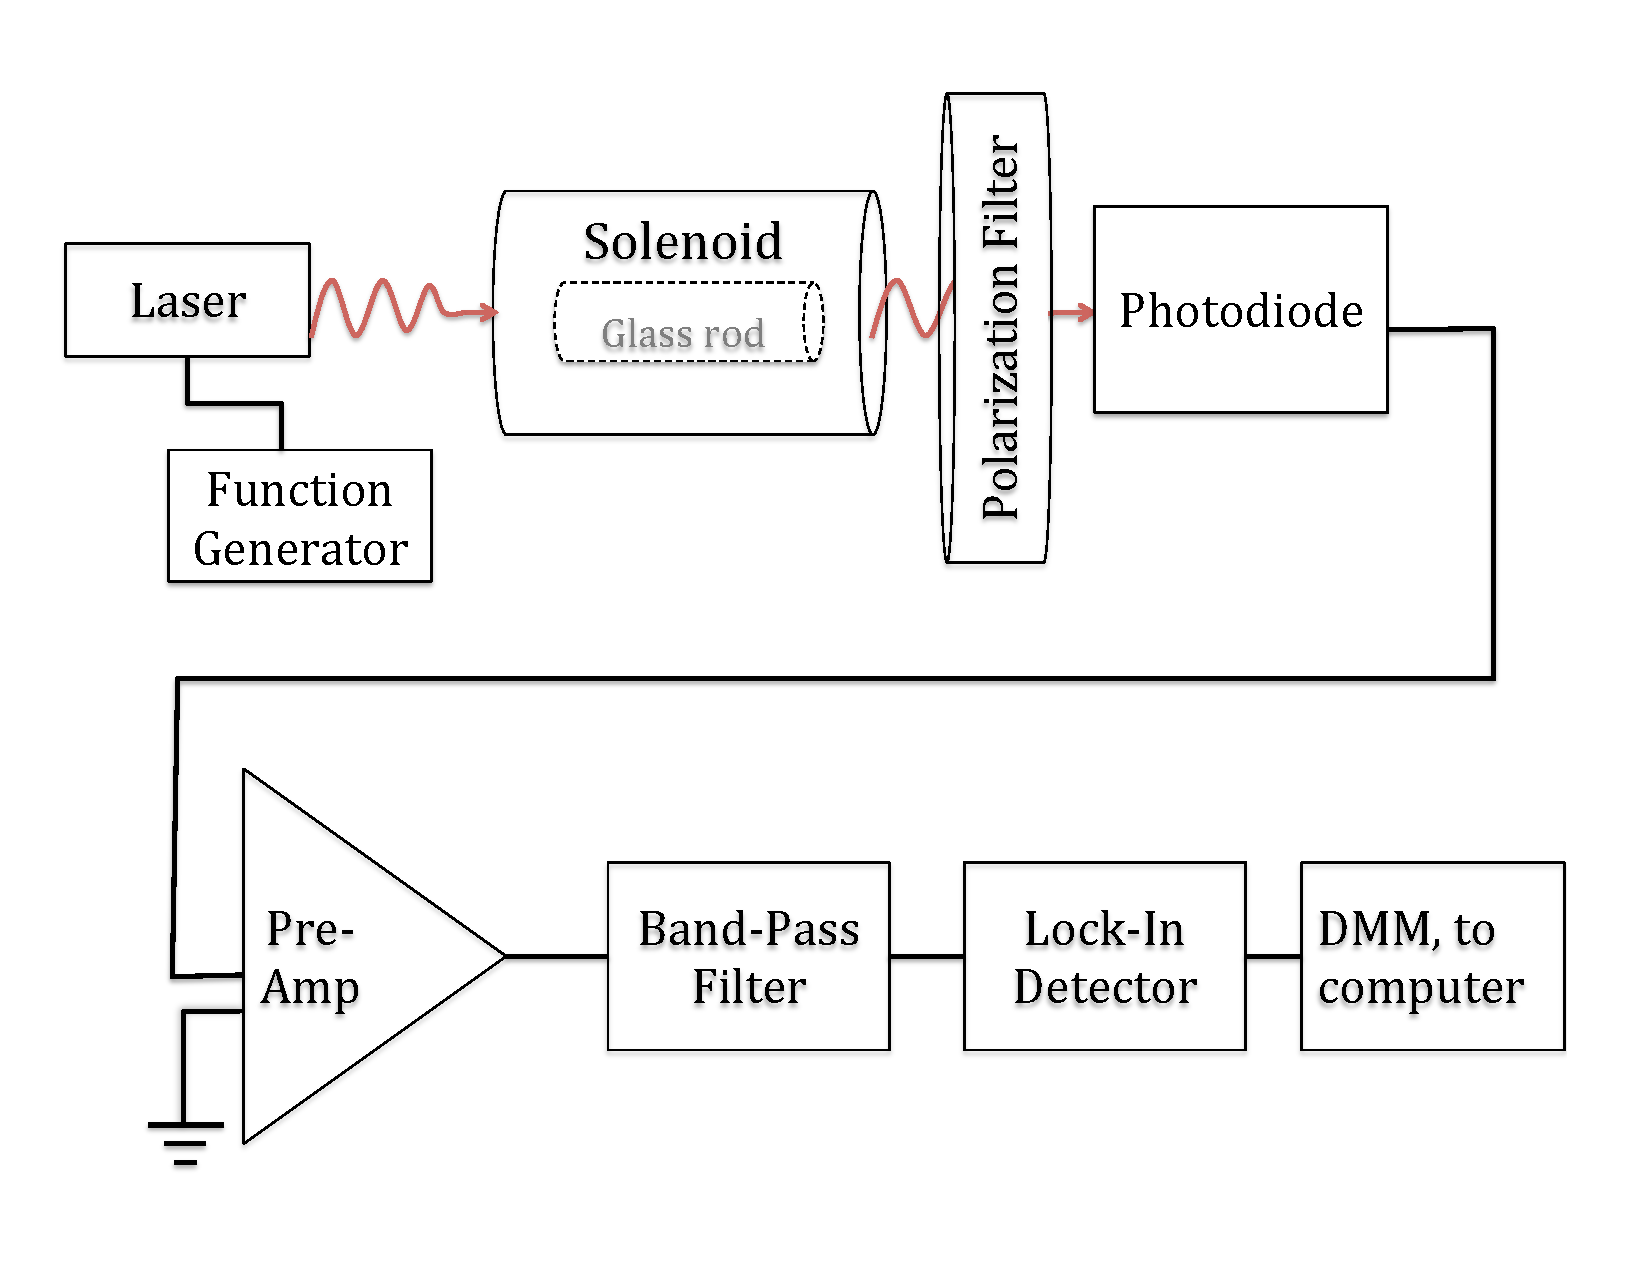
\includegraphics[width=6in]{Faraday_lab_set-up.pdf}
\caption{The set-up of our experiment. The light source was a laser, modulated by a function generator. We sent the beam through a solenoid containing a rod of material, and next a polarization filter. A photodetector at the other end measured the light intensity. This signal went through a  lock-in detector, and from there to the computer.}
\label{set-up}
\end{figure}


Our power source was a XXXXX which we used on current control throughout our experiment. We connected the two 3 volt ??  terminals in parallel so that we could obtain a total current of 3 amps through the solenoid. By varying the current through the solenoid we could change the magnetic field through the XXXXX rod. We measured the magnetic field using a XXXXX for a current of 2A and obtained a field of 21.8mT at the center of solenoid decreasing to 20.5mT at the edges of the XXXX rod. We took the average of this rage to be our best value and difference between high and low values divided by two to be our uncertainty. To obtain field values for other currents we exploited the linear relationship between magnetic field and current.
We used a Keithley XXXX function generator to modulate the laser at at frequency of XXXXX. The signal from the photodiode was run through a preamp, a bandpass filter and a lock-in detector. We used lock-in detector to stabilize our measurements and filter out ambient light from the room along with other forms of systematic error.
The output from the lock-in detector was then measured with a Keithley XXXX DMM. To facilitate data collection we used a computer program (helpfully provided by our instructors) called "Keithley DC Incremental Write." The program would record 16 values for voltage, average them and give the result with uncertainty as one data point. 
For our changing theta experiment, we measured the voltage while rotating the polarizing lens. We started with no current and an angle of 90\deg between the polarized laser and the polarizing lens, so that our intensity (and measured voltage) was at a minimum. This was our relative angle of 0\deg. We then measured the voltage every 10\deg for a single rotation (360\deg). We repeated this this measurement for currents of I = 1A, I = 2A and I = 3A.
For our changing field experiment, we set our relative angle to 45\deg we then measured the voltage for currents 0A, \pm1A, \pm2A and \pm3A. For this experiment we set the computer program to average over 100 values for each data point.

\section{Results}

We performed the experiment to measure the Verdet constant of our material in two different ways, and so obtained two different sets of data.  From the measurement of light intensity due to changing polarization filter angle in a constant magnetic field, for currents of 0A, 1A, 2A, and 3A, we obtained the results shown in Figure ~\ref{V_ThetaRel_Plot}. 

\begin{figure}[h!]
\centering
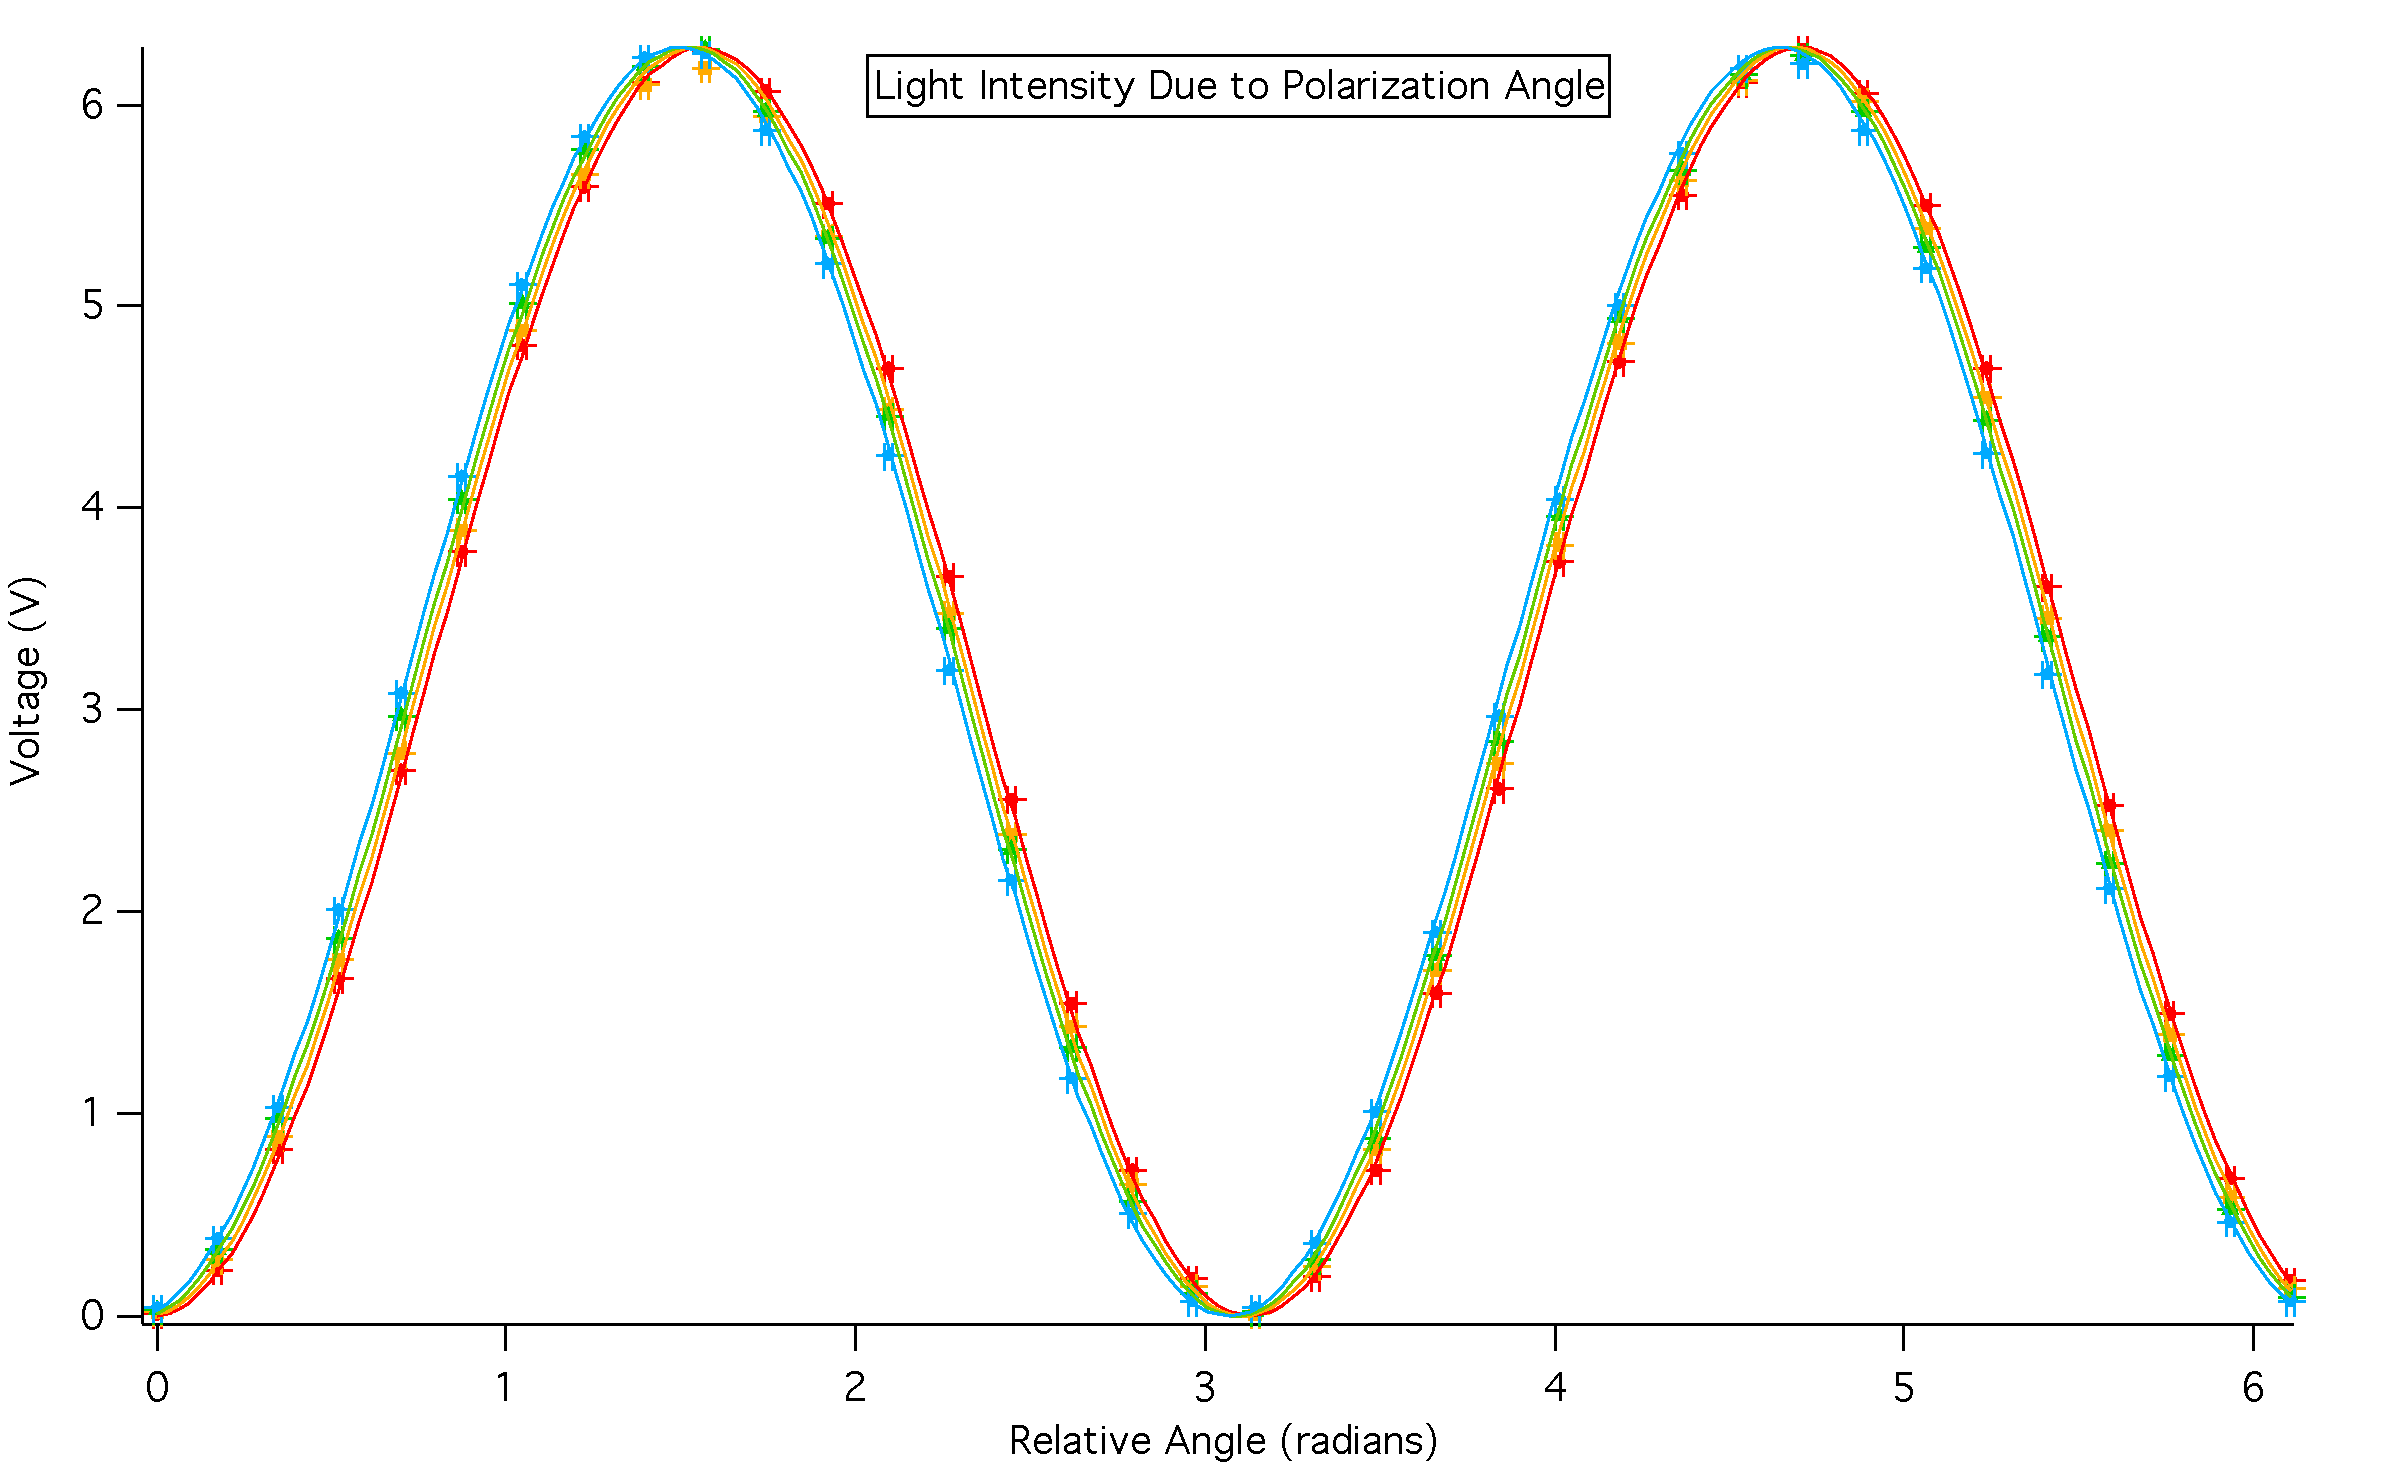
\includegraphics[width=6in]{V_ThetaRel_Plot.pdf}
\caption{Photo-detector voltage (proportional to light intensity) plotted against relative angle (the angle between the filter and the laser’s polarization) from 0 to 2pi radians.  The red points are the measurements taken without a magnetic field, the orange points were taken with 1A of current passing through the solenoid, the green points with the current at 2A, and the blue points at 3A.  The curve fits are the function $V = A \cos^{2}(\theta + C) – A$, with $A$ held constant at 6.2845 V (obtained from the first curve fit), and $C$ calculated by the curve fit. }
\label{V_ThetaRel_Plot}
\end{figure}

From the measurements of changing magnetic field, with a constant polarization filter angle, for currents from -3A to 3A in steps of 0.5A, we obtained the results shown in Table ~\ref{V_I_Table}. 

\begin{table}[h!]
\centering
\caption{Voltage readings from the photodetector for various currents applied to the solenoid. }
\begin{ruledtabular}
\begin{tabular}{c c c}
Current (A) & Voltage (V) & Error Voltage (V)\\
\hline	% horizontal line to separate headings from data
-3   & 2.822 & 1.30E-10 \\
-2.5 & 2.887 & 5.47E-10 \\
-2   & 2.951 & 3.72E-10 \\
-1.5 & 3.016 & 3.78E-11 \\
-1   & 3.082 & 8.98E-10 \\
-0.5 & 3.145 & 9.03E-10 \\
0    & 3.211 & 1.18E-09 \\
0.5  & 3.272 & 1.16E-10 \\
1    & 3.338 & 2.05E-09 \\
1.5  & 3.404 & 2.13E-09 \\
2    & 3.468 & 6.96E-10 \\
2.5  & 3.534 & 1.12E-09 \\
3    & 3.599 & 1.05E-09
\end{tabular}
\end{ruledtabular}
\label{V_I_Table}
\end{table}

\section{Analysis}

%I'm putting our figures and tables here for later

\begin{table}[h!]
\centering
\caption{The fields due to the currents in table ~\ref{V_I_Table} applied to our solenoid, with the resulting voltage measured by the photodetector. }
\begin{ruledtabular}
\begin{tabular}{c c c c}
Magnetic Field * Length (mT*cm) & Error B*L (mT*cm) & Voltage (V) & Error Voltage (V)\\
\hline	% horizontal line to separate headings from data
-323 & 12 & 2.822 & 1.30E-10 \\
-269 & 10 & 2.887 & 5.47E-10 \\
-215 & 8  & 2.951 & 3.72E-10 \\
-161 & 6  & 3.016 & 3.78E-11 \\
-108 & 4  & 3.082 & 8.98E-10 \\
-54  & 2  & 3.145 & 9.03E-10 \\
0    & 0  & 3.211 & 1.18E-09 \\
54   & 2  & 3.272 & 1.16E-10 \\
108  & 4  & 3.338 & 2.05E-09 \\
161  & 6  & 3.404 & 2.13E-09 \\
215  & 8  & 3.468 & 6.96E-10 \\
269  & 10 & 3.534 & 1.12E-09 \\
323  & 12 & 3.599 & 1.05E-09
\end{tabular}
\end{ruledtabular}
\label{V_B*L_Table}
\end{table}

\begin{table}[h!]
\centering
\caption{C values taken from the curve fits to Figure ~\ref{V_ThetaRel_Plot}}
\begin{ruledtabular}
\begin{tabular}{c c c}
Current (A) & C value from curve fit (rad) & Error C value (rad)\\
\hline	% horizontal line to separate headings from data
0 & 0.0088553 & 0.001  \\
1 & 0.030849  & 0.0014 \\
2 & 0.049599  & 0.0013 \\
3 & 0.072754  & 0.0015
\end{tabular}
\end{ruledtabular}
\label{I_cValue_Table}
\end{table}

\begin{table}[h!]
\centering
\caption{Calculated phase shifts for the changing angle experiment, with the magnetic fields calculated from the applied currents.}
\begin{ruledtabular}
\begin{tabular}{c c c c}
Phase Shift (rad) & Error Phase Shift (rad) & Magnetic Field*Length (mT*cm) & Error Magnetic Field*Length (mT*cm)\\
\hline	% horizontal line to separate headings from data
0 & 0.002  & 0  & 0  \\
0.022  & 0.0024 & 108 & 4  \\
0.0407 & 0.0023 & 215 & 8  \\
0.0639 & 0.0025 & 323 & 12
\end{tabular}
\end{ruledtabular}
\label{B*L_PhaseShift_Table}
\end{table}

\begin{figure}[h!]
\centering
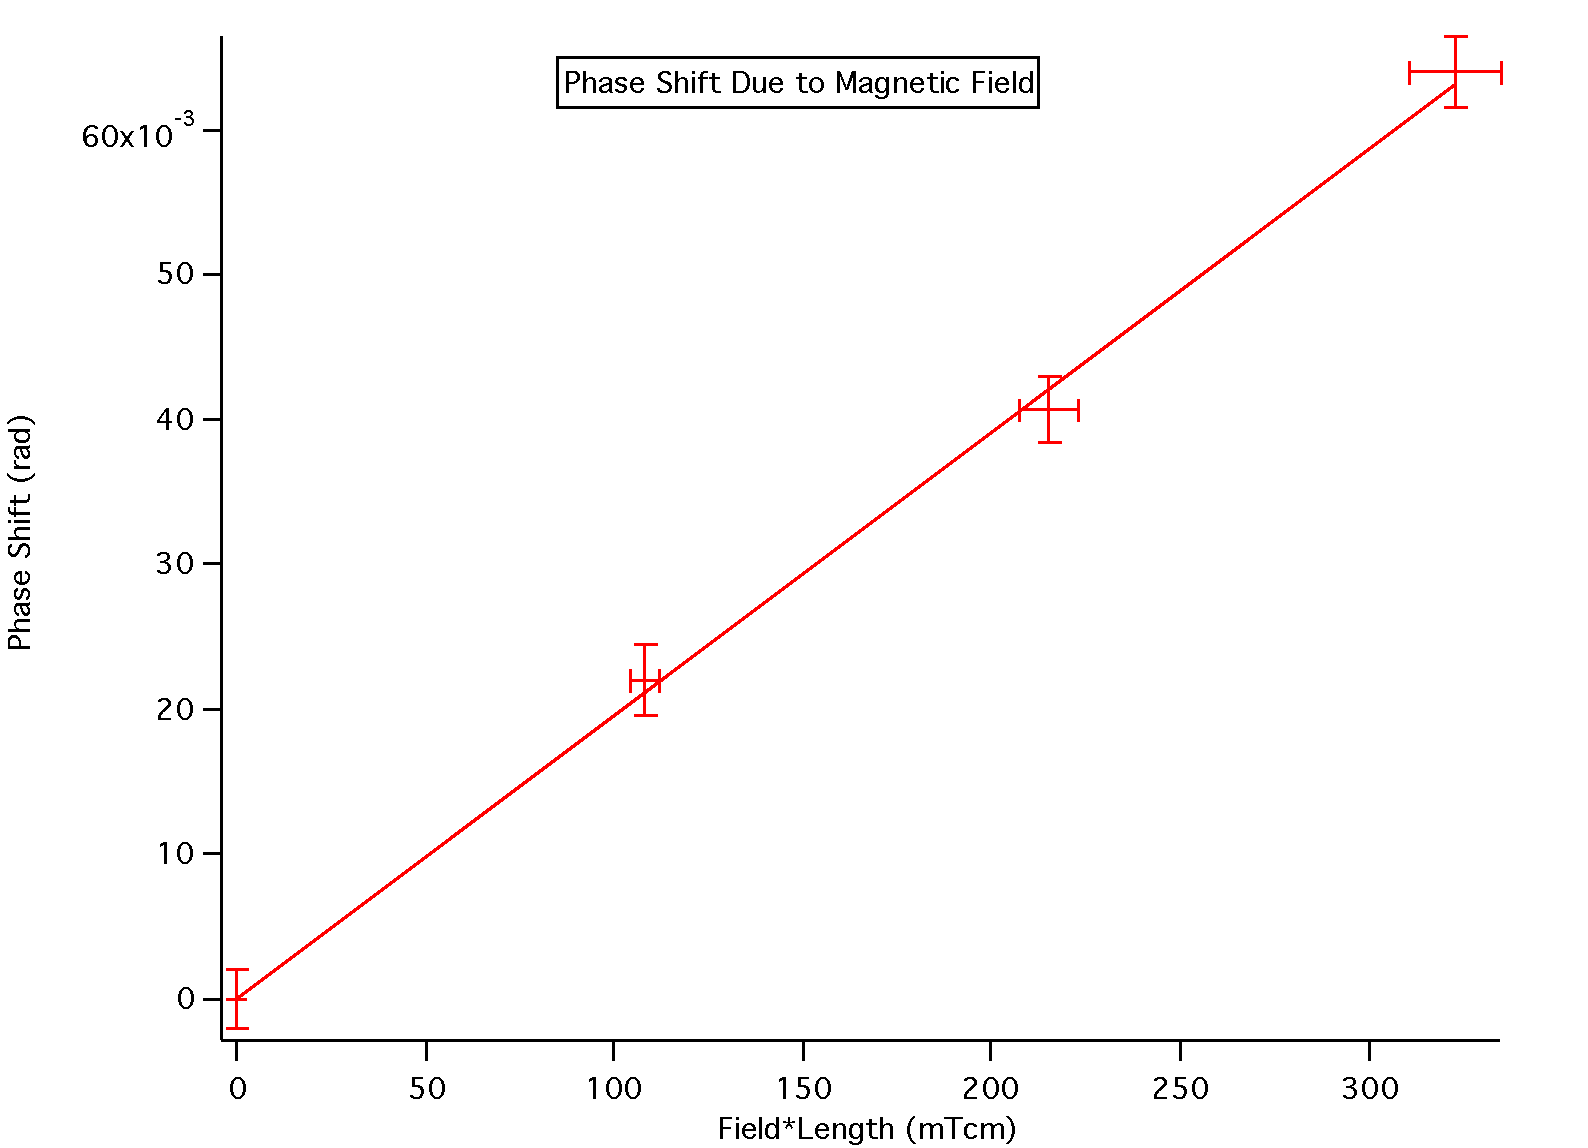
\includegraphics[width=5in]{PhaseShift_B-L_Plot.pdf}
\caption{A plot of Table \ref{B*L_PhaseShift_Table}, applied magnetic field (times length of the refracting material) versus the resulting phase shift in the polarization of the laser beam. The slope of a linear curve fit of this plot gives a value for the verdet constant of the material. }
\label{PhaseShift_B*L_Plot}
\end{figure}

\begin{figure}[h!]
\centering
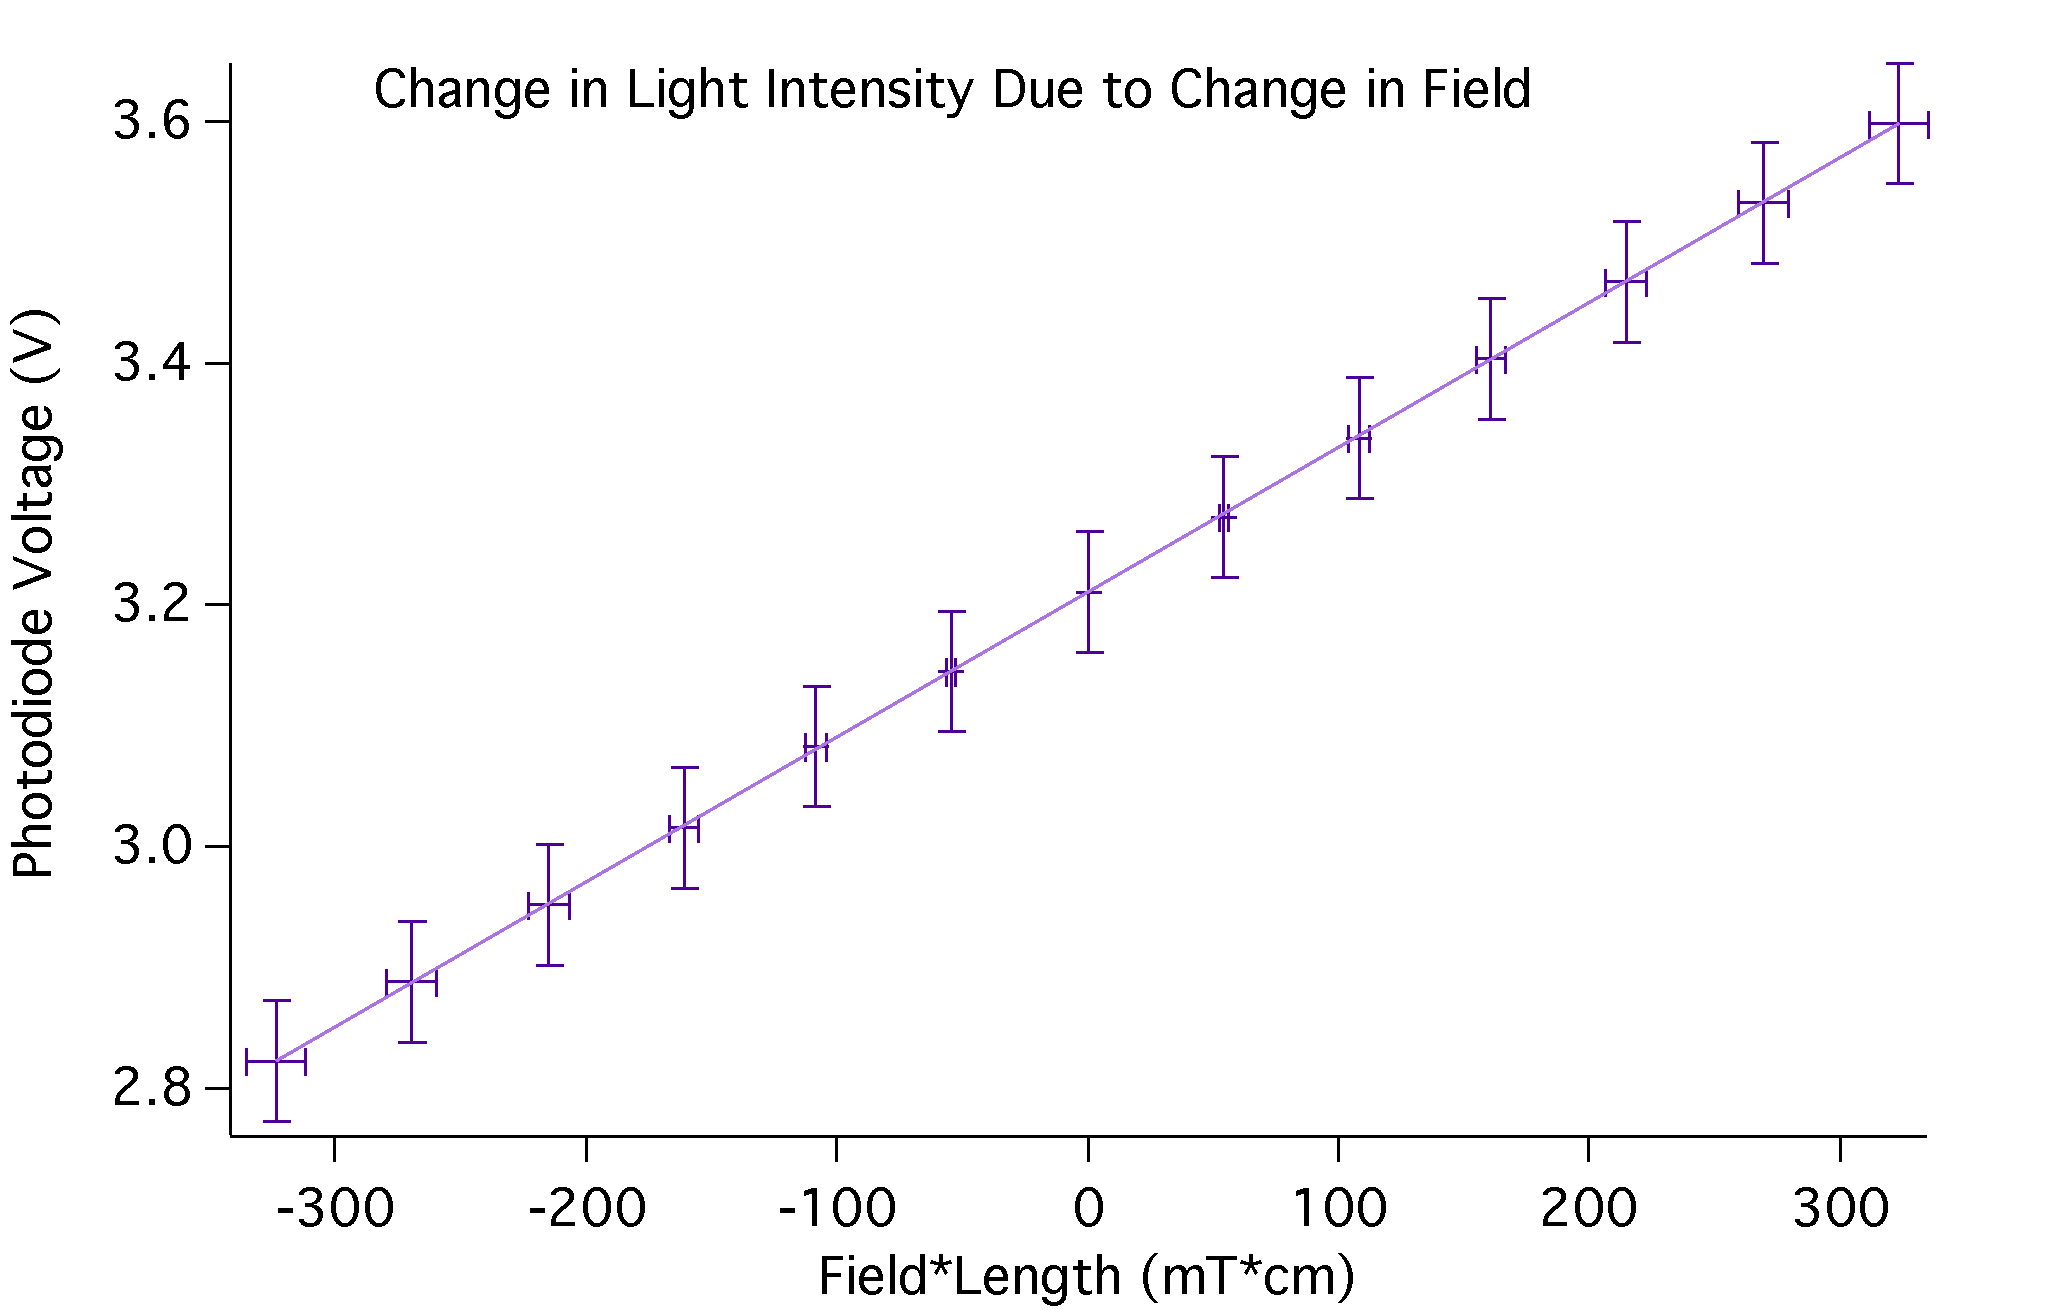
\includegraphics[width=5in]{V_B-L_Plot.pdf}
\caption{A plot of Table \ref{V_B*L_Table}, the applied magnetic field (times the length of the refracting material) versus the voltage measured by the photodetector for that field. The slope of a linear curve fit to this plot can be used to calculate the verdet constant of the material. }
\label{V_B*L_Plot}
\end{figure}

\section{Discussion}

\section{Conclusion}

\end{document}
